%%%%%%%%%%%%%%%%%%%%%%%%%%%%%%%%%%%%%%%%%
% Wenneker Assignment
% LaTeX Template
% Version 2.0 (12/1/2019)
%
% This template originates from:
% http://www.LaTeXTemplates.com
%
% Authors:
% Vel (vel@LaTeXTemplates.com)
% Frits Wenneker
%
% License:
% CC BY-NC-SA 3.0 (http://creativecommons.org/licenses/by-nc-sa/3.0/)
% 
%%%%%%%%%%%%%%%%%%%%%%%%%%%%%%%%%%%%%%%%%

%----------------------------------------------------------------------------------------
%	PACKAGES AND OTHER DOCUMENT CONFIGURATIONS
%----------------------------------------------------------------------------------------

\documentclass[11pt]{scrartcl} % Font size

%%%%%%%%%%%%%%%%%%%%%%%%%%%%%%%%%%%%%%%%%
% Wenneker Assignment
% Structure Specification File
% Version 2.0 (12/1/2019)
%
% This template originates from:
% http://www.LaTeXTemplates.com
%
% Authors:
% Vel (vel@LaTeXTemplates.com)
% Frits Wenneker
%
% License:
% CC BY-NC-SA 3.0 (http://creativecommons.org/licenses/by-nc-sa/3.0/)
% 
%%%%%%%%%%%%%%%%%%%%%%%%%%%%%%%%%%%%%%%%%

%----------------------------------------------------------------------------------------
%	PACKAGES AND OTHER DOCUMENT CONFIGURATIONS
%----------------------------------------------------------------------------------------

\usepackage{amsmath, amsfonts, amsthm} % Math packages

\usepackage{listings} % Code listings, with syntax highlighting

\usepackage[english]{babel} % English language hyphenation

\usepackage{graphicx} % Required for inserting images
\graphicspath{{Figures/}{./}} % Specifies where to look for included images (trailing slash required)

\usepackage{booktabs} % Required for better horizontal rules in tables

\numberwithin{equation}{section} % Number equations within sections (i.e. 1.1, 1.2, 2.1, 2.2 instead of 1, 2, 3, 4)
\numberwithin{figure}{section} % Number figures within sections (i.e. 1.1, 1.2, 2.1, 2.2 instead of 1, 2, 3, 4)
\numberwithin{table}{section} % Number tables within sections (i.e. 1.1, 1.2, 2.1, 2.2 instead of 1, 2, 3, 4)

\setlength\parindent{0pt} % Removes all indentation from paragraphs

\usepackage{enumitem} % Required for list customisation
\setlist{noitemsep} % No spacing between list items

%----------------------------------------------------------------------------------------
%	DOCUMENT MARGINS
%----------------------------------------------------------------------------------------

\usepackage{geometry} % Required for adjusting page dimensions and margins

\geometry{
	paper=a4paper, % Paper size, change to letterpaper for US letter size
	top=2.5cm, % Top margin
	bottom=3cm, % Bottom margin
	left=3cm, % Left margin
	right=3cm, % Right margin
	headheight=0.75cm, % Header height
	footskip=1.5cm, % Space from the bottom margin to the baseline of the footer
	headsep=0.75cm, % Space from the top margin to the baseline of the header
	%showframe, % Uncomment to show how the type block is set on the page
}

%----------------------------------------------------------------------------------------
%	FONTS
%----------------------------------------------------------------------------------------

\usepackage[utf8]{inputenc} % Required for inputting international characters
\usepackage[T1]{fontenc} % Use 8-bit encoding

\usepackage{fourier} % Use the Adobe Utopia font for the document

%----------------------------------------------------------------------------------------
%	SECTION TITLES
%----------------------------------------------------------------------------------------

\usepackage{sectsty} % Allows customising section commands

\sectionfont{\vspace{6pt}\centering\normalfont\scshape} % \section{} styling
\subsectionfont{\normalfont\bfseries} % \subsection{} styling
\subsubsectionfont{\normalfont\itshape} % \subsubsection{} styling
\paragraphfont{\normalfont\scshape} % \paragraph{} styling

%----------------------------------------------------------------------------------------
%	HEADERS AND FOOTERS
%----------------------------------------------------------------------------------------

\usepackage{scrlayer-scrpage} % Required for customising headers and footers

\ohead*{} % Right header
\ihead*{} % Left header
\chead*{} % Centre header

\ofoot*{} % Right footer
\ifoot*{} % Left footer
\cfoot*{\pagemark} % Centre footer
 % Include the file specifying the document structure and custom commands

%----------------------------------------------------------------------------------------
%	TITLE SECTION
%----------------------------------------------------------------------------------------

\title{	
	\normalfont\normalsize
	\textsc{Sharif University of Technology, Electrical Engineering Department}\\ % Your university, school and/or department name(s)
	\vspace{25pt} % Whitespace
	\rule{\linewidth}{0.5pt}\\ % Thin top horizontal rule
	\vspace{20pt} % Whitespace
	{\huge Project 1: Jenkin’s Governor}\\ % The assignment title
	\vspace{12pt} % Whitespace
	\rule{\linewidth}{2pt}\\ % Thick bottom horizontal rule
	\vspace{12pt} % Whitespace
}

\author{\LARGE Ali Seyfi \and \LARGE Vahid Ahmadi}
 


\date{\normalsize\today} % Today's date (\today) or a custom date

\begin{document}

\maketitle % Print the title

%----------------------------------------------------------------------------------------
%	FIGURE EXAMPLE
%----------------------------------------------------------------------------------------

\section{governor problem sets}

\begin{figure}[h] % [h] forces the figure to be output where it is defined in the code (it suppresses floating)
	\centering
	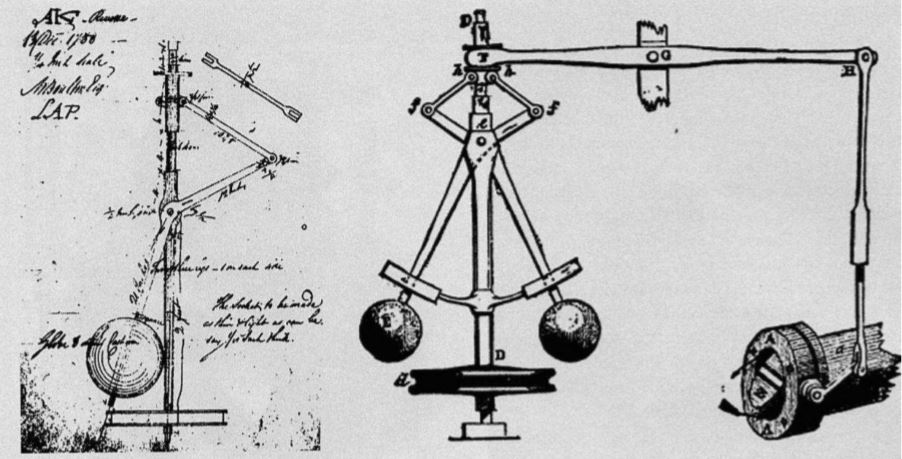
\includegraphics[width=0.7\columnwidth]{images/p1.JPG} % Example image
	\caption{Flyball Governor invented by James Watt in 1788.}
\end{figure}

%------------------------------------------------

\subsection{Derive the equations for $\psi$ and $\theta$ using the free body diagrams shown in Figure $1.2 .$ Combine these two to obtain the differential equation of velocity $w(\dot{\theta})$.}

Let $\theta$ be the rotation angle of the principal axis, $m$ be the mass of a flyball, $k$ be the spring constant, $r$ be the distance between the flyball and the center of the axis of rotation, and $V_{1}$ be the lowest limit of the angular velocity at which the friction ring starts to rotate. At the velocity $V_{1}$, the flyballs begin to rub against the inside of the friction ring, and the centrifugal force and spring force are balanced at this speed
\begin{equation}m r_{1} V_{1}^{2}=k\left(r_{1}-r_{0}\right)\end{equation}
The Maxwell torque linearized it to be
\begin{equation}F\left(\dot{\theta}-V_{1}\right)\end{equation}
By assuming that the velocity $\dot{\theta}$ varies within very narrow limits around the value $V_{1} .$ That is, by assuming
%%%%%%%%%\begin{equation}\dot{\theta} \triangleq V_{1}+\dot{\theta}\end{equation}
Then we have
\begin{equation}F=4 r_{1}^{2} \mu m V_{1}\end{equation}
The differential equation for the rotation $\theta$ of the principal axis is
\begin{equation}M \ddot{\theta}=P-R-F\left(\dot{\theta}-V_{1}\right)-G \psi\end{equation}
where $P$ is the driving torque; $R$ is the resisting torque; $G$ is a constant; $\psi$ is the rotation angle of the friction ring; and $M$ is the total moment of inertia of the principal axis, brake drum, and all the rotating parts with respect to the principal axis. From the free-body diagram in Figure $10(\mathrm{b})$ the equation of motion of the friction ring is
\begin{equation}B \ddot{\psi}=F\left(\dot{\theta}-V_{1}\right)-Y \dot{\psi}-W\end{equation}

\begin{figure}[h] % [h] forces the figure to be output where it is defined in the code (it suppresses floating)
	\centering
	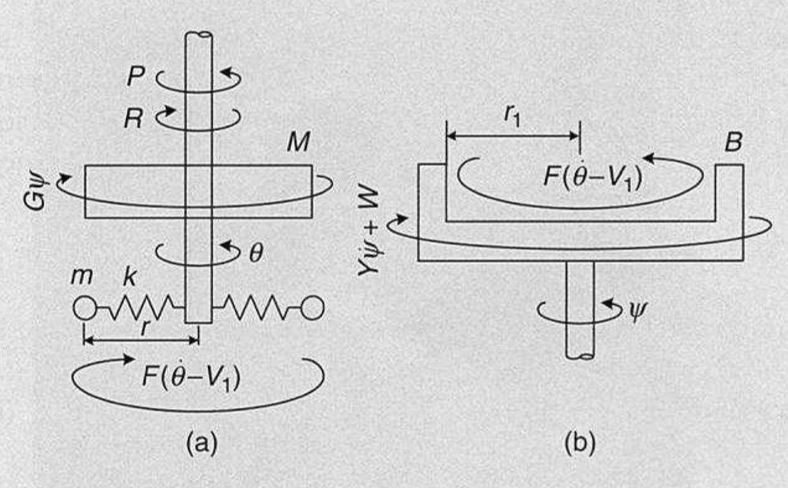
\includegraphics[width=0.5\columnwidth]{images/p2.JPG} % Example image
	\caption{A free body diagram of Jenkin's Governor.}
\end{figure}
%----------------------------------------------------------------------------------------

\subsection{Linearize your model assuming that the velocity $\dot{\theta}$ varies within very narrow bound around the $V 1$ That is, by assuming $\dot{\theta}=V 1+\Delta \dot{\theta}$.}

where $B$ is the total moment of inertia of the friction ring and the attached parts, $Y$ is a coefficient corresponding to viscous friction torque due to the hydraulic cylinder, and $W$ is a constant torque acting on the friction ring owing to the weight. Equations of motion derived by Maxwell, except that Maxwell called $\theta$ and $\psi, x$ and $y,$ respectively. Linear differential equation that is third order in the velocity $\omega(=\dot{\theta})$ is 
\begin{equation}
M B \ddot{\omega}+(M Y+F B) \ddot{\omega}+F Y \dot{\omega}+F G \omega=u(t)
\end{equation}
Where input $u(t)$ is
\begin{equation}
u(t)=B(\ddot{P}-\ddot{R})+Y(\dot{P}-\dot{R})+G F V_{1}+G W
\end{equation}
For constant $P$ and $R,$ Maxwell obtained a solution of the form
\begin{equation}
\omega(t)=A_{1} e^{s_{1} t}+A_{2} e^{s_{2} t}+A_{3} e^{s_{3} t}+V
\end{equation}
Where $V$ is the nominal velocity given by
\begin{equation}
V=V_{1}+W / F
\end{equation}
At the steady state we have
\begin{equation}
G F V=G F V_{1}+G W
\end{equation}

\subsection{Find the stability condition for the model you have derived in the previous section using Routh's array, explain how system parameters affect the stability.}

$s_{1}, s_{2}, s_{3}$ are the roots of the cubic characteristic equation
\begin{equation}
M B s^{3}+(M Y+F B) s^{2}+F Y s+F G=0
\end{equation}
Maxwell obtained the stability condition that the real roots and the real parts of the complex conjugate roots of the characteristic equation $(1.12)$ must all be negative. He presented the stability condition as
\begin{equation}
\left(\frac{F}{M}+\frac{Y}{B}\right) \frac{Y}{B}-\frac{G}{B}=\text { positive value }
\end{equation}

Using Routh's array:
\[
\begin{array}{lc}
s^{3}: M B & F Y \\
s^{2}: M Y+F B & F G \\
s: \frac{(M Y+F B) F Y-(M B)(F G)}{M Y+F B} & \\
1: F G &
\end{array}
\]
For stability, all elements of the first column of the Routh array must be positive.
All coefficients in equation below must be positive:
\begin{equation}
M B s^{3}+(M Y+F B) s^{2}+F Y s+F G=0
\end{equation}
They are actually positive until parameters are physical values.

\subsection{In Jenkin's governor the centrifugal piece is at a constant distance from the axis of rotation. However, there are other kinds of governor in which the centrifugal piece is free to move from the axis of rotation but is balanced by a centrifugal force and the force of gravity (or by the spring force, in some cases).\newline
$(a) .$ Name an example of this alternative type of Governor system.\newline
$(b) .$ Explain how this difference can affect the stability conditions of the system.}
$(a) .$ 
\begin{enumerate}
	\item Sir William Thomson and Léon Foucault governor model.
	\item Watt's Centrifugal Governor model Figure $1.3 $. 
\end{enumerate}
\begin{figure}[h] 
	\centering
	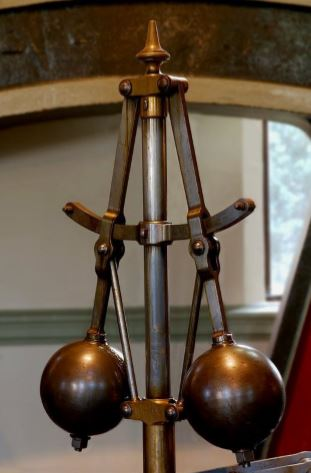
\includegraphics[width=0.3\columnwidth]{images/p3.JPG} 
	\caption{Watt's Centrifugal Governor.}
\end{figure}
$(b) .$ \newline
Let’s solve for a famous example model: Sir William Thomson and Léon Foucault governor model. Maxwell expressed the equations of motion using the angular momentum $A \dot{\theta}$
\begin{equation}
\frac{d}{d t}(A \dot{\theta})=L
\end{equation}
Where $\theta$ is the angle of revolution about the vertical axis, $A$ is the moment of inertia of a revolving apparatus for $\theta$ motion, and $L$ is the total torque acting on the axis. Let $B$ be the moment of inertia of the flyballs in Figure $1.4 $ for $\phi$ motion. Then, the sum of the kinetic and potential energies of Foucault's governor is
\begin{equation}
E=\frac{1}{2} A \dot{\theta}^{2}+\frac{1}{2} B \dot{\phi}^{2}+P=\int L d \theta
\end{equation}
Where $P$ is the potential energy of the apparatus, which is a function of the divergence angle $\phi$ of the centrifugal piece. Here, $A$ and $B$ are both functions of the angle $\phi$. We can rearrange the equation:
\begin{equation}
\frac{d}{d t}(B \phi)=\frac{1}{2} A_{\phi}\left(\theta^{2}-V^{2}\right)+\frac{1}{2} B_{\phi} \phi^{2}
\end{equation}
By assuming:
%%%%%\begin{equation} \theta \triangleq V+\omega, \quad \phi \triangleq \phi_{1}+\phi \end{equation}
Also, the linear differential equations are:
\begin{equation}
\begin{array}{l}
A \omega+A_{\phi} V \phi=L \\
B \phi-A_{\phi} V \omega=0
\end{array}
\end{equation}
To convert this apparatus into a governor, the equations become:
\begin{equation}
A \omega+X \omega+K \phi+G \phi=L
\end{equation}
\begin{equation}
B \phi+Y \phi-K \omega=0
\end{equation}
After model Linearization we have:
\begin{equation}
A B \phi+(A Y+B X) \phi+\left(X Y+K^{2}\right) \phi+G K \phi=L
\end{equation}
So, the stability condition of equation is (confirmed by the Routh stability criterion):
\begin{equation}
\left(\frac{X}{A}+\frac{Y}{B}\right)\left(X Y+K^{2}\right)>G K
\end{equation}
\begin{figure}[h] 
	\centering
	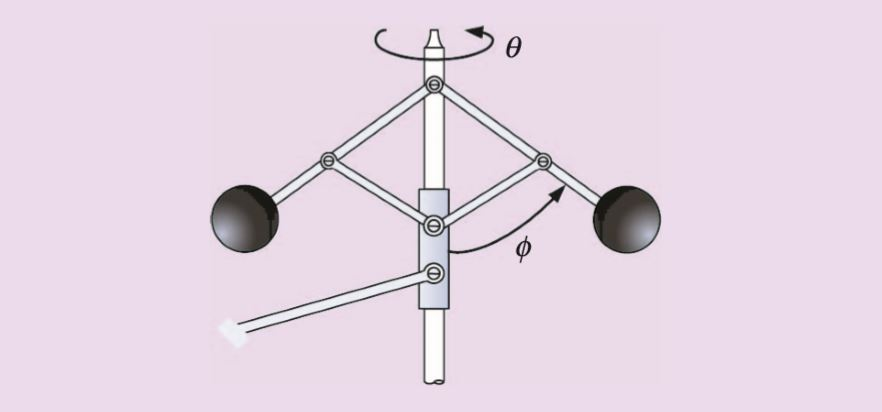
\includegraphics[width=0.5\columnwidth]{images/p4.JPG}
	\caption{The centrifugal pieces (that is, flyballs) of Foucault’s governor.}
\end{figure} \newpage
\subsection{Draw a block diagram of the Governor control loop. Specify the actuator, controller input and controller output and name all signals.}
\begin{figure}[h] 
	\centering
	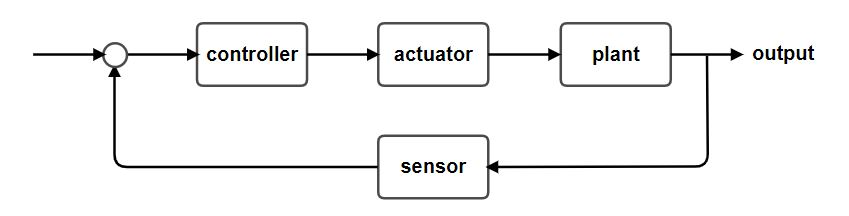
\includegraphics[width=0.8\columnwidth]{images/p5.JPG}
	\caption{General close loop (feedback) control system.}
\end{figure} \newpage



\subsection{Simulate the system using Simulink based on the model you have derived in the previous section. Choose reasonable values for your parameters and justify your choices in your report.}
\subsection{Identify the time constant of the system. Experiment with different values of $m, r, k .$ Explain the impact of the above-mentioned parameters on the system's performance. Justify your observations.}

















\end{document}
